\chapter{GEM detector Data Analysis}

Gas Electron Multiplier(GEM) Detectors are gaseous detectors. The key component of the GEM detector is 5um copper-coated polyimide foils. On the foil, there are 70um holes are etched in a regular hexagonal pattern, and the distance between that holes is 140 micrometers. On the top of the GEM foil is the cathode, and under the bottom is the readout board used for collecting the employed electrons. A potential difference applied across the foils generates sharp electric fields in the holes. The electrons created during the ionization process drift toward the foils and are multiplied in the holes. The resulting electron avalanche induces a readout signal on the finely spaced strips. To achieve a higher amplify ability, multiple layers of GEM detector are stacked together, and with those layers of GEM foils, the ionized electron can be amplified multiple times before reaches the readout board. 

The GEM detectors used for PRex/CRex experiment were designed for Jefferson Lab Super BigBite Spectrometer(SBS) with an area of 50cmx60cm. By the time it was built, it was one of the largest GEM detectors that have ever been built. The PRex/CRex provides a good opportunity to test the GEM detector in a real experiment environment before the start of the SBS experiment. It will provide a good supplement when the event rate is high since VDC efficiency drops or even does not work at high event rate.  In this chapter, we will cover the apparatus and the analysis result of the GEM detectors. 


\section{GEM detector}

The SBS GEM detector used in PRex/CRex experiment consists of three layers of GEM foils. On top of the GEM foil is the cathode, it has a similar structure as GEM foil with holes on the foil, but instead of double side cooper coated, the cathode is single-side coated. On top of the GEM foil is a thin layer of an aluminized gas window that applies the same high voltage as the cathode to avoid polarization because of the charges on the cathode. 

The gas in the GEM detector is pre-mixed $75\%$ Argon and $25\%$ Carbon Dioxide provided by the Hall A gas system. The mixed gas first comes into the chamber between the entrance window and the cathode and then passes through the hold of the foil which could provide a unified mixture of the gas throughout the whole chamber.  The exhaust gas  comes out from the exhaust holes on the frame from the bottom of the GEM chamber. 

On the bottom of the GEM foils, the avalanche electrons are collected with 2d readout strips. Each of the readout strips is connected to one channel of charge-sensitive pre-amplify electronics. To avoid the bend of the readout board because of the mixed gas in the chamber, another chamber is designed under the readout board, and filled with Air with exactly the same pressure as the GEM chambers. 

\begin{figure}[!tbp]
  \centering
  \begin{minipage}[b]{0.45\textwidth}
    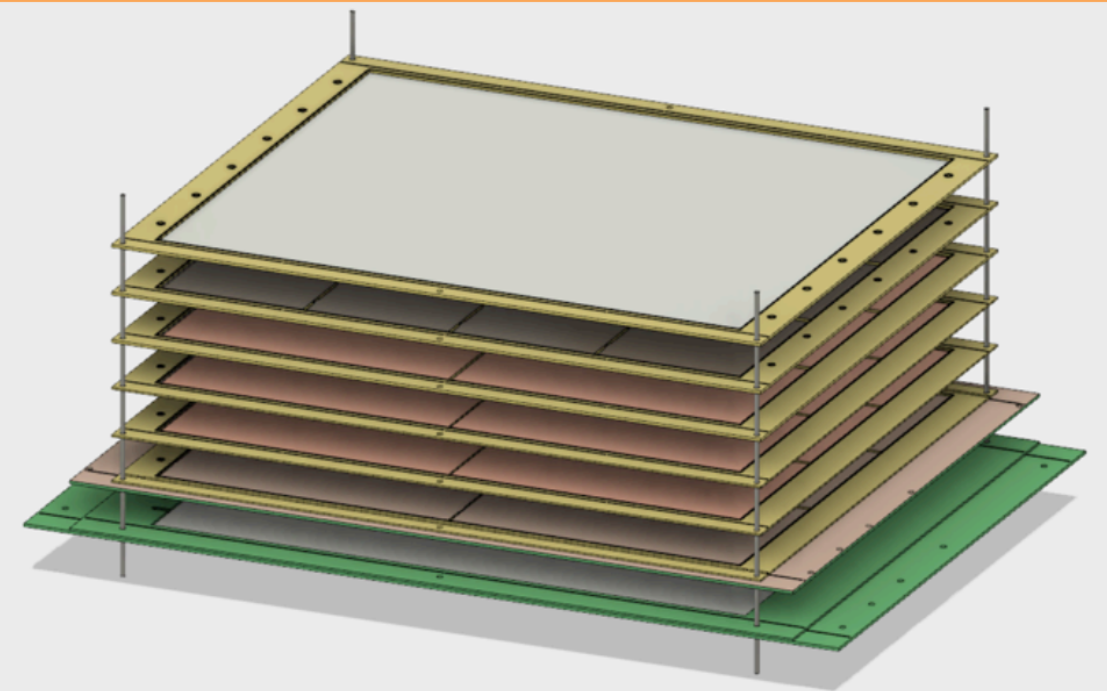
\includegraphics[width=\textwidth]{images/chap5/gem_structure_3d.png}
    \caption{GEM Chamber 2D structure}
  \end{minipage}
  \hfill
  \begin{minipage}[b]{0.45\textwidth}
    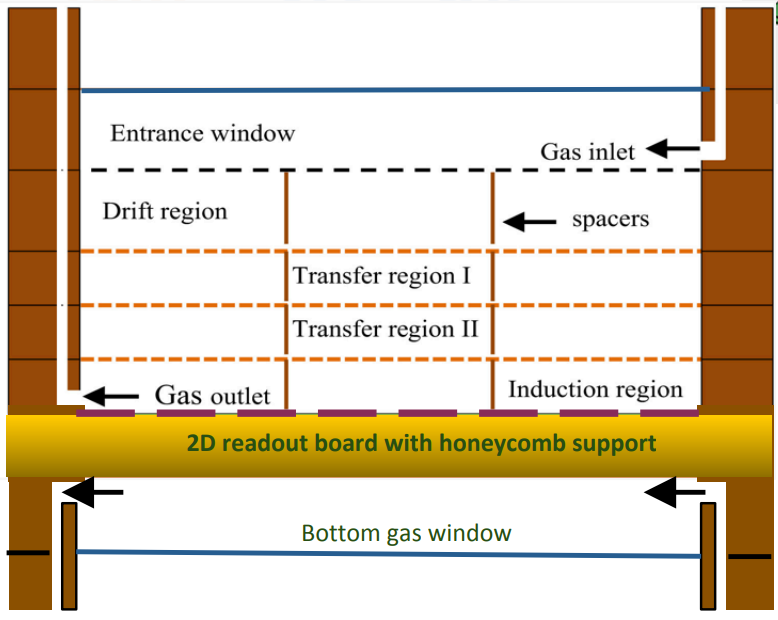
\includegraphics[width=\textwidth]{images/chap5/gem_structure_chamber_2d.png}
    \caption{GEM chamber Gas flow}
  \end{minipage}
\end{figure}

\subsection{GEM detector structure}
\begin{itemize}
    \item GEM foil
    \item GEM structure 
    \item GEM readout board
    \item GEM readout electronics
\end{itemize}
\subsection{GEM detector in apparatus}
\begin{itemize}
    \item GEM detector in the shell
    \item GEM detector in the HRS
\end{itemize}
\section{GEM detector data analysis}
\subsection{the procedure used to get the GEM signals}
\subsection{pedestal}
\begin{itemize}
    \item how to get the pedestal
    \item pedestal False Positive Rate Study
\end{itemize}
\subsection{GEM detector alignment}
\subsection{GEM detector performance}
\begin{itemize}
    \item GEM detector cluster size
    \item GEM detector number of strips fired
    \item GEM detector tracking efficiency
    \item GEM detector efficiency over time 
    \item GEM detector High Rate Performance and compare with VDC 
\end{itemize}
